\documentclass{article}
\usepackage{mathtools}
\usepackage{backnaur}
\usepackage{multirow}
\usepackage{hhline}
\usepackage{textgreek}
\usepackage{setspace}
\doublespacing

\renewcommand{\bnfpo}{\Coloneqq}

\usepackage{fullpage}
\usepackage{logicproof}
\usepackage{parskip}
\usepackage{forest}
\usepackage{float}
\usepackage{hyperref}
\usepackage{colortbl, xcolor}

\definecolor{Red}{rgb}{1,0.8,0.8}

\newcommand{\imp}{\ensuremath{\rightarrow}}
\newcommand{\seq}{\ensuremath{\vdash}}
\newcommand{\ent}{\ensuremath{\models}}
\newcommand{\elim}{\ensuremath{\mathit{e}}}
\newcommand{\intr}{\ensuremath{\mathit{i}}}
\newcommand{\rep}[1]{copy #1}

% p116
\newcommand{\landi}[2]{$\land_\intr$ #1, #2}
\newcommand{\landex}[1]{$\land_{\elim_1}$ #1}
\newcommand{\landey}[1]{$\land_{\elim_2}$ #1}
\newcommand{\lorix}[1]{$\lor_{\intr_1}$ #1}
\newcommand{\loriy}[1]{$\lor_{\intr_2}$ #1}
\newcommand{\lore}[5]{$\lor_\elim$ #1, #2--#3, #4--#5}

% p117
\newcommand{\impi}[2]{$\imp_\intr$ #1--#2}
\newcommand{\impe}[2]{$\imp_\elim$ #1, #2}

% p118
\newcommand{\negi}[2]{$\neg_\intr$ #1--#2}
\newcommand{\nege}[2]{$\neg_\elim$ #1, #2}

% p119
\newcommand{\bote}[1]{$\bot_\elim$ #1}
\newcommand{\nnege}[1]{$\neg\neg_\elim$ #1}

% p120
\newcommand{\nnegi}[1]{$\neg\neg_\intr$ #1}

% 122
\newcommand{\modt}[2]{$\mathit{MT}$ #1, #2}

% 123
\newcommand{\pbc}[2]{$\mathit{PBC}$ #1--#2}

% 124
\newcommand{\lem}{\ensuremath{\mathit{LEM}}}

% formula logic
\newcommand{\fneg}[1]{\ensuremath{\left(\neg #1 \right)}}
\newcommand{\fland}[2]{\ensuremath{\left( #1 \land #2 \right)}}
\newcommand{\flor}[2]{\ensuremath{\left( #1 \lor #2 \right)}}
\newcommand{\fimp}[2]{\ensuremath{\left( #1 \imp #2 \right)}}

% formula logic, parenthesis override
\newcommand{\Fneg}[1]{\ensuremath{\neg #1}}
\newcommand{\FlanD}[2]{\ensuremath{#1 \land #2}}
\newcommand{\Fland}[2]{\ensuremath{#1 \land \left( #2 \right)}}
\newcommand{\flanD}[2]{\ensuremath{\left( #1 \right) \land #2}}
\newcommand{\FloR}[2]{\ensuremath{#1 \lor #2}}
\newcommand{\Flor}[2]{\ensuremath{#1 \lor \left( #2 \right)}}
\newcommand{\floR}[2]{\ensuremath{\left( #1 \right) \lor #2}}
\newcommand{\FimP}[2]{\ensuremath{#1 \imp #2}}
\newcommand{\Fimp}[2]{\ensuremath{#1 \imp \left( #2 \right)}}
\newcommand{\fimP}[2]{\ensuremath{\left( #1 \right) \imp #2}}

\newcommand{\true}{\textbf{true}}
\newcommand{\false}{\textbf{false}}

\edef\restoreparindent{\parindent=\the\parindent\relax}
\usepackage{parskip}
\restoreparindent

\title{CMPE 58S: Sp. Tp. Computer Aided Verification \\ Project: Interactive Propositional Logic Engine using Natural Deduction}
\date{\today{}}
\author{Mehmet Utkan Gezer \\ 2018700060}

\begin{document}
\maketitle

\section{Introduction}

Propositional logic, also known as propositional calculus, is the branch
of logic dealing with propositions. Natural deduction is a way of handling
propositions, whereby we apply a collection of rules to infer new
conclusions from zero or more premises, all of which themselves are
propositions.

For a more detailed introduction, we will be giving some definitions for
propositions and natural deduction, along with its semantics.

\subsection{Propositions}\label{sec:intr_prop}

Propositions are declarative
sentences with a truth value either \true{} or \false{},
and can be recursively defined as the composition of
some other, smaller, propositions. Smallest of propositions are
called \textit{atomic} propositions, which are \textit{indecomposable}
and are given a unique symbol for the declarations they make.

\textit{Compositionals} are propositions composed of other propositions,
i.e. propositions that are not atomic. In propositional logic, there
are 4 different ways of composing a \textit{compositional}:

\begin{enumerate}
	\item Negation ($\neg$): Negation of a proposition. E.g.
		``it does not rain'' is the negation of ``it rains''.
		If the original proposition has the truth value
		\true{}/\false{}, then its negation has the truth value
		\false{}/\true{}, respectively.
	\item Conjunction ($\land$): Conjunction of two propositions. E.g.
		``it does not rain and I am 25'' is the conjunction of the propositions
		``it does not rain'' and ``I am 25''. The compositional has
		the truth value \true{} only if both of its constituents
		have the truth value \true{}, and otherwise \false{}.
	\item Disjunction ($\lor$): Disjunction of two propositions. E.g.
		the non-exclusive sense of the statement
		``it is sunny or I am 5'' is the conjunction of the propositions
		``it is sunny'' and ``I am 5''. The compositional has the truth
		value \false{} only if both of its constituents have the truth
		value \false{}, otherwise (if either one or both of its constituents
		have the truth value \true{}) the compositional is \true{}.
	\item Implication ($\imp$): Implication of the second proposition,
		also known as the \textit{consequent}, by the first proposition,
		also known as the \textit{antecedent}. E.g.
		``if it is sunny then I am happy'' is the implication of
		the proposition ``I am happy'' by the proposition ``it is sunny''.
		The compositional has the truth value \false{} only if the
		antecedent and consequent are \true{} and \false{}, respectively.
\end{enumerate}

To formally define the \textit{language} of propositional logic's
\textit{well-formed formulas}, we give its Backus Naur form (BNF)
as follows:

\begin{bnf*}
	\bnfprod{$\phi$}
	{
		\bnfpn{atom} \bnfor
		\bnfts{$\Big(\neg$} \bnfpn{$\phi$} \bnfts{$\Big)$} \bnfor
		\bnfts{$\Big($} \bnfpn{$\phi$} \bnfts{$\land$}
			\bnfpn{$\phi$} \bnfts{$\Big)$} \bnfor
		\bnfts{$\Big($} \bnfpn{$\phi$} \bnfts{$\lor$}
			\bnfpn{$\phi$} \bnfts{$\Big)$} \bnfor
		\bnfts{$\Big($} \bnfpn{$\phi$} \bnfts{$\imp$}
			\bnfpn{$\phi$} \bnfts{$\Big)$}
	}\\
	\bnfprod{atom}
	{
		\bnfts{$p$} \bnfor \bnfts{$q$} \bnfor \bnfts{\bnfsk} \bnfor
		\bnfts{$p_1$} \bnfor \bnfts{$p_2$} \bnfor \bnfts{\bnfsk}
	}
\end{bnf*}

While this definition requires each use of a compositional operator
to introduce a new pair of parenthesis for the newly generated
proposition to be a well-formed formula, in practice we encounter
propositons with many of those parenthesis omitted. In absence of
parenthesis to enforce an explicit precedence of operator application,
following precedence conventions are consulted:

\begin{itemize}
	\item $\neg$ binds most tightly, followed by $\land$, $\lor$, and
		finally $\imp$, in the given order.
	\item Implication ($\imp$) is right-associative, i.e. the
		rightmost implication is to be evaluated the first.
\end{itemize}

Some books, including \textit{Logic in Computer Science} by Huth and
Ryan~\cite{huth2004logic},
regard $\land$ and $\lor$ operations as equal in precedence, in which
case a proposition like $p \lor q \land r$ should either be regarded
as unintelligible, or the same as $((p \lor q) \land r)$.
We will be adhering to the above listed convention.

\subsection{Natural deduction}\label{sec:intr_nd}

Natural deduction is a way of reasoning about a given set of propositions
and inferring new ones from them. Using a collection of \textit{proof rules},
natural deduction allows us to come up with \textit{conclusions} starting
off by a set of \textit{premises}. This relation between premises and
conclusions are formalized by expressions called \textit{sequents},
such as:
$$
\phi_1, \phi_2, \dotsc, \phi_n \vdash \psi.
$$

Sequents with no premises are also valid sequents, and are called
\textit{theorems}.

Rules of natural deduction, also known as the previously mentioned
proof rules, are at the heart of natural deduction, and this project.
They allow us to establish a valid proof step with a proposition,
using the previously validated list of propositions.

At any step, we may introduce an \textit{assumption} to the proof,
which, however, will introduce an assumption box along with it.
The top line of the assumption box is drawn right above the step
at which the assumption is introduced. We may close the assumption
box after any step. A proof rule may only be applied to propositions,
such that;
\begin{itemize}
	\item Their validity must have been previously established, and
	\item Either they must be outside any assumption box, or their
		assumption box must not have been closed, yet.
\end{itemize}

We refer to such proof steps as the \textit{accessible steps}.

A proof of a sequent is complete when the conclusion of the
sequent is established using only the rules of natural deduction and
starting off with only the premises of the sequent. It is important to
note that an established proposition may not be the conclusion if it is
found within an \textit{assumption box}.

Here is a list of all natural deduction rules we have embedded into
our program, given in sequents:

\begin{center}
	\renewcommand{\arraystretch}{1.2}
	\newcommand{\nl}{\\[4pt]}
	\newcommand{\nll}{\\[4pt]\hline}
	\begin{tabular}{l l|l}
		\multicolumn{2}{l|}{\textbf{Name}} & \textbf{Rule}\\\hhline{==|=}
		\multirow{3}{*}{Conjunction}
		& Introduction    & $\phi, \psi \vdash \phi \land \psi$\nl
		& Elimination \#1 & $\phi \land \psi \vdash \phi$\nl
		& Elimination \#2 & $\phi \land \psi \vdash \psi$\nll
		\multirow{3}{*}{Disjunction}
		& Introduction \#1 & $\phi \vdash \phi \lor \psi$\nl
		& Introduction \#2 & $\psi \vdash \phi \lor \psi$\nl
		& Elimination      & $\phi \lor \psi, \boxed{\phi \dotsb \chi},
			\boxed{\psi \dotsb \chi} \vdash \chi$\nll
		\multirow{2}{*}{Implication}
		& Introduction & $\boxed{\phi \dotsb \psi} \vdash \phi \implies \psi$\nl
		& Elimination  & $\phi \implies \psi, \phi \vdash \psi$\nll
		\multirow{2}{*}{Negation}
		& Introduction & $\boxed{\phi \dotsb \bot} \vdash \neg\phi$\nl
		& Elimination  & $\phi, \neg\phi \vdash \bot$\nll
		\multirow{1}{*}{\false{}}
		& Elimination  & $\bot \vdash \phi$\nll
		\multirow{2}{*}{Double negation}
		& Introduction & $\phi \vdash \neg\neg\phi$\nl
		& Elimination  & $\neg\neg\phi \vdash \phi$\nll
		\multicolumn{2}{l|}{MT (Modus Tollens)}
		& $\phi \imp \psi, \neg\psi \vdash \neg\phi$\nll
		\multicolumn{2}{l|}{PBC (Proof by Contraditcion)}
		& $\boxed{\neg\phi \dotsb \bot} \vdash \phi$\nll
		\multicolumn{2}{l|}{LEM (Law of Excluded Middle)}
		& $\vdash \phi \lor \neg\phi$\nll
		\multicolumn{2}{l|}{Copy}
		& $\phi \vdash \phi$
	\end{tabular}
\end{center}

The boxed premises such as $\boxed{\phi \dotsb \psi}$ on
implication introduction, is an assumption box in the proof
that starts right before the proposition $\phi$ and ends right
after the proposition $\psi$. 
To make step on the proof, one of the proof rules given
above must be used. To use a rule, we need accessible propositions
and/or assumption boxes that fits to the rule's sequent's propositions.
Only if we are able to fulfill the \textit{requirements} of the rule,
we then may establish the validity of a new proposition according
to the definition of the rule, and specifically the rule's sequent's
conclusion. In natural deduction, this is the only way to
make a proof step and approach to the ultimate conclusion.

Accessibility of an assumption box is defined similar to the
accessibility of individual proof steps. This time, not a single
step but the assumption box as a whole should be accessible as a
single entity.

A proof step is a declaration, and should have a \textit{rationale}
stated next to it. Following is a complete list of valid rationales
for a proof step:
\begin{center}
	\begin{tabular}{r | p{37em}}
		\textbf{Rationale} & \textbf{Can be used next to propositions which\ldots{}}\\\hline
		Premise: & \ldots{} are found in the premises of the sequent to be proved.\\
		Proof rule: & \ldots{} that fit to the conclusion of a proof rule, and only if the
			corresponding premises of that proof rule is available and validated in a
			previous step. Those steps must be referenced in the rationale in the
			same order as they appear in the proof rule.\\
		Assumption: & \ldots{} appear as the first proof step of an assumption box.
	\end{tabular}
\end{center}

Here is an example of a proof for the sequent
$p \lor q, \neg q \lor r \seq p \lor r$:

\begin{figure}[H]
	\begin{logicproof}{2}
		p \lor q                & premise\\
		\neg q \lor r           & premise\\
		q \lor \neg q           & \lem\\
		\begin{subproof}
			q                   & assumption\\
			\begin{subproof}
				\neg q          & assumption\\
				\bot            & \nege{4}{5}\\
				r               & \bote{6}
			\end{subproof}
			\begin{subproof}
				r               & assumption
			\end{subproof}
			r                   & \lore{2}{5}{7}{8}{8}\\
			p \lor r            & \loriy{9}
		\end{subproof}
		\begin{subproof}
			\neg q              & assumption\\
			\begin{subproof}
				p               & assumption
			\end{subproof}
			\begin{subproof}
				q               & assumption\\
				\bot            & \nege{13}{11}\\
				p               & \bote{14}
			\end{subproof}
			p                   & \lore{1}{12}{12}{13}{15}\\
			p \lor r            & \lorix{16}
		\end{subproof}
		p \lor r                & \lore{3}{4}{10}{11}{17}
	\end{logicproof}
	\caption{Proof for the sequent $p \lor q, \neg q \lor r \seq p \lor r$.}
	\label{fig:proof}
\end{figure}

And here are remarks on this proof:
\begin{enumerate}
	\item Note that on step \#3, we use the rule \lem{} without
		any argument. It really does not depend on any one of the
		previous steps, however, it actually has an argument $q$,
		which is the reason why it is a rationale for $q \lor \neg q$
		and not $\neg r \lor \neg\neg r$.
	\item Note the order of arguments on step \#14. With respect to the
		rule of negation elimination ($\neg_\elim$), second of its two
		arguments must be the negation-applied of the first one, which
		is why we first refer to $q$ and then $\neg q$, and not the other
		way around. Also note that negation-applied is not the same
		as negation-discarded, although they semantically have the same meaning.
	\item Note how assumption boxes are referred to with ranges, i.e.
		the starting index, followed by a dash, and followed by the ending index.
\end{enumerate}

Hereby we conclude with our definitions on propositional logic
and natural deduction, and also our introduction.

\section{Interactive Propositional Logic Engine using Natural Deduction}

A \textit{propositional logic engine} is an abstract machine that
works with propositional logic as its substance. One that works
with the methods of natural deduction, is a propositional logic
engine \textit{using natural deduction}. With this project,
we propose an \textit{interactive} propositional logic engine
using natural deduction.

Our product is a software that allows its user to build up valid proofs
for any given propositional logic sequent. By stating the rule they
want to use and specifying the arguments that want to use it with,
users can establish the truth of newer propositions and get them added
to the proof as a step. The proof rules are embedded into the software,
ensuring the validity of the proof throughout the execution.

The software comes with a command-line interface, which is a REPL%
\footnote{Read-Eval-Print-Loop}
that reads user input for proof rules, parses and evaluates it, and
re-draws the working proof to the console window, in a loop. The
loop ends when the conclusion of the initially input sequent is reached.

In the following sections, we will be giving out more details on
software's workflow, its the input specifications and some of its
inner mechanisms. We will also mention some of its software design
aspects, some of which have been made possible (with ease) of the
programming language Julia.

\subsection{Workflow}

At all times, the program greets the user with the title same as the
name of the project, ``Interactive Propositional Logic Engine using
Natural Deduction''. Initially, the program asks user to provide
a sequent that is to be proven.

After being provided a sequent, the program enters the proof mode,
where it will start displaying a working proof structure with step
numbers and box visualizations with ASCII box characters for the
assumption boxes. In this mode, the user is repeatedly asked to
provide a natural deduction rule to apply. With the provided
natural deduction rule, along with its parameters, the software
will do either one of the following:
\begin{itemize}
	\item If the rule is applicable to the given arguments, it will
		add the proposition, validity of which has been established
		using the provided proof rule with the given arguments, and
		then re-draw the proof with the new step on the proof.
	\item If the rule is malformed:
		\begin{itemize}
			\item The program may ask the user to re-consider their
				input, or
			\item The program may fail and exit.
		\end{itemize}
\end{itemize}

The program is designed to apply a properly provided natural
deduction rule, and only apply a properly provided natural deduction
rule. However, as stated above, it may fail to recover promptly
and ask for the user to retry if an input is malformed.

Apart from the natural deduction rules with their parameters,
some other keyword statements can be provided to the program
to perform the closure of an assumption box, and, for user's
convenience, to undo the last action.

When a proof step with the proposition exactly the same as in the
conclusion of the initially provided sequent and outside all of
the assumption boxes, the program than declares success and
exits. This concludes the workflow of the program, and also this
section.

\subsection{Input specifications}

Our program accepts 3 different category of inputs:
Propositions, sequents, and natural deduction statements
with their arguments. We will provide their specifications
separately for a more structured view.

\subsubsection{Propositions}

Refer to the Section~\ref{sec:intr_prop} for the BNF specification
for the well-formed formulas on propositions. As stated before
in that section, we will not expect the user-provided formulas
to be well-formed, and tolerantly accept propositions according
to precedence rules described in again the same section.

In general, and with respect to the BNF specification, a proposition
consists of atoms, negation, conjunction, disjunction, and implication
symbols, and finally parenthesis. We extend this list of constituents with
constants for tautology and contradiction, which we have seen to take
place in propositions, both in the proof rules and the example we gave.

Since we cannot expect users to input Unicode characters like $\land$
for the \textbf{and} operation, we instead accept sensible ASCII
alternatives to represent these operations. We do not accept the
Unicode originals, even if the user somehow manages to type them down.
Here is the full list of those alternatives, next to their Unicode
originals:

\begin{center}
	\begin{tabular}{c | c c}
		\multirow{2}{*}{\textbf{Unicode}} & \multicolumn{2}{c}{\textbf{\underline{Alternative}}}\\
		& \textbf{\#1} & \textbf{\#2}\\
		\hline
		$\mathtt{\top}$  & \verb|T|                & \verb|TRUE|\\
		$\mathtt{\bot}$  & \verb|F|                & \verb|FALSE|\\
		$\mathtt{\neg}$  & \verb|!|                & \\
		$\mathtt{\land}$ & \verb|&|                & \verb|*|\\
		$\mathtt{\lor}$  & \verb^|^                & \verb|+|\\
		$\mathtt{\imp}$  & \verb|->|               & \\
		$\mathtt{()}$    & \verb|()|               & \verb|[]|\\
		$\mathtt{q_1}$   & \verb|q1|               &
	\end{tabular}
\end{center}

Atomic propositions which are symbolized with a single letter should simply
be input using that letter. Atoms with a subscript number should have their
number appended right next to them, and not as a subscript. More specifically,
all the atoms should be in the form of the following regular expression:

\begin{center}
\verb|[a-z][0-9]*|
\end{center}

There can be as many spaces around the tokens as the user may input,
as well as no space at all. A couple of example propositions our program
would accept are as follows:

\begin{center}
	\begin{tabular}{l | l}
		\verb^(((!p) & q) -> (p & (q | (!r))))^ & \verb^(p1 -> (p2 -> (p3 -> p4)))^\\
		\verb^!p & q -> p & (q | !r)^           & \verb^p1 -> p2 -> p3 -> p4^\\
		\verb^!p&q   ->   p&((q)|!r)^           & \verb^(((p1->p2->p3->p4)))^
	\end{tabular}
\end{center}

All 6 of the inputs are valid, and the ones on the same column are
two different ways of writing the same proposition. The top ones are
explicit and well-formed formulas, while the remaining 4 are dependent
on conventions of precedence. The bottom ones are untidy examples, where
there are a superfluous spaces and then sometimes none. Last examples
also exhibit extra parenthesis, which are adequately handled by the
parenthesis elimination routine in our program.

\subsubsection{Sequents}

Refer to the Section~\ref{sec:intr_nd} for the definitions of a sequent.
Recall that a sequent with no premises is also a valid sequent, also known
as a theorem.

List of premises in a sequent are to be separated with commas (\verb|,|)
in our program, just like we do it on paper. The symbol $\vdash$ should
be substituted by \verb|=>|.  If the user desires to provide a theorem,
the sequent symbol \verb|=>| can also be omitted altogether.

Conclusion of the sequent may not be omitted, as it is essential for a
sequent. However, if the user desires to use the program for natural deduction
without any pre-destined conclusion, he or she may simply provide an unattainable
conclusion, such as an atomic proposition \verb|q1234| that does not take place
in any one of the premises. This should allow them to run the program
indefinitely, as it should be impossible for them to establish the validity
of an atomic proposition that does not exist in any one of the premises.

As with the propositions, there can be as many spaces around the tokens as
the user feels like, as well as no space at all. A couple of example sequents
our program would accept are as follows:

\begin{center}
	\begin{tabular}{l}
		\verb^!q -> !p => p -> !!q^\\
		\verb^p -> (q -> r), p, !r => !q^\\
		\verb^p -> q -> r  , p  , !r=>!q^\\
		\verb^=> (q -> r) -> ((!q -> !p) -> (p -> r))^\\
		\verb^(q -> r)   ->  ((!q -> !p) -> (p -> r))^
	\end{tabular}
\end{center}

Here, second and third, and fourth and fifth sequents are equivalent, i.e.
will be interpreted as the same by our program.

\subsubsection{Natural deduction statements}\label{sec:spec_nd}

\textit{Natural deduction rules} have no syntax, but they are rather rules to be
applied to true propositions in order to establish the truth of newer ones. When a
proposition is introduced using a natural deduction rule, however, we have to
specify the rule as a rationale next to that proposition in a very specific way.

\newcommand{\AN}{\texttt{\#}}
\newcommand{\AR}{\texttt{\#-\#}}
\newcommand{\AF}{\texttt{\textphi}}

In our program, we adopt this rationale syntax, as we expect user to provide
\textit{natural deduction statements}. In general, a natural deduction statement
should start with the identifier of the corresponding natural deduction rule,
followed by the list of parameters it takes. Here, parameters are either one of
the following three:
\begin{itemize}
	\item Line number, with the placeholder \AN.
	\item An interval of line numbers, with the placeholder \AR.
	\item A proposition, with the placeholder \AF.
\end{itemize}

The following table specifies all of the natural deduction statements that our
program accepts: First two columns are the names of the statements, and corresponds
to the names of the natural deduction rules. The next column is the identifier for
the statement, and the following columns are placeholders for one of the three
different types of parameters as listed above.

The last 3 statements on the table are the only ones that do not have a corresponding
natural deduction rule. First two are there to open and close assumption boxes,
and the last one is for the convenience of the user, allowing them to undo the effects
of the last (non-\verb|undo|) statement they have provided.

\begin{center}
	\renewcommand{\arraystretch}{1}
	\begin{tabular}{l l|l|l l l}
		\multicolumn{2}{l|}{\multirow{2}{*}{\textbf{Name}}}
		& \multirow{2}{*}{\textbf{Identifier}}
		& \multicolumn{3}{c}{\textbf{\underline{Arguments}}} \\
		& &
		& \textbf{\#1}
		& \textbf{\#2}
		& \textbf{\#3}\\\hhline{==|=|===}
		\multirow{3}{*}{Conjunction}
		& Introduction    & \verb|andi|  & \AN & & \\
		& Elimination \#1 & \verb|ande1| & \AN & & \\
		& Elimination \#2 & \verb|ande2| & \AN & & \\\hline
		\multirow{3}{*}{Disjunction}
		& Introduction \#1 & \verb|ori1| & \AN & \AF & \\
		& Introduction \#2 & \verb|ori1| & \AN & \AF & \\
		& Elimination      & \verb|ori1| & \AN & \AR & \AR \\\hline
		\multirow{2}{*}{Implication}
		& Introduction & \verb|impi| & \AR & & \\
		& Elimination  & \verb|impe| & \AN & \AN & \\\hline
		\multirow{2}{*}{Negation}
		& Introduction & \verb|negi| & \AR & & \\
		& Elimination  & \verb|nege| & \AN & \AN & \\\hline
		\multirow{1}{*}{\false{}}
		& Elimination  & \verb|bote| & \AN & \AF & \\\hline
		\multirow{2}{*}{Double negation}
		& Introduction & \verb|negnegi| & \AN & & \\
		& Elimination  & \verb|negnege| & \AN & & \\\hline
		\multicolumn{2}{l|}{MT (Modus Tollens)}
		& \verb|MT| & \AN & \AN & \\\hline
		\multicolumn{2}{l|}{PBC (Proof by Contraditcion)}
		& \verb|PBC| & \AR & & \\\hline
		\multicolumn{2}{l|}{LEM (Law of Excluded Middle)}
		& \verb|LEM| & \AF & & \\\hline
		\multicolumn{2}{l|}{Copy}
		& \verb|copy| & \AN & & \\\hline
		\multicolumn{2}{l|}{Assume}
		& \verb|assume| & \AF & & \\\hline
		\multicolumn{2}{l|}{Conclude}
		& \verb|conclude| & & & \\\hline
		\multicolumn{2}{l|}{Undo}
		& \verb|undo| & & &
	\end{tabular}
\end{center}

The \AN{} should be replaced by a single line number out of one of the
line numbers that are present in the working proof so far. \AR{} should
be replaced by two line numbers separated by a dash (\verb|-|), where
the first line number should be of the line right after the start of
an assumption box opening line, and the second line number should be of
the line right before the end of an assumption box closing line. 
The \AF{} should be replaced by any proposition, as previously described
at the propositions' input specification.

The user may separate the identifier from the first argument either with
one or more space characters (\verb| |), or a comma (\verb|,|)
with any amount of space characters around it. The arguments should also
be separated from each other in a similar fashion.

All the arguments are necessary, and the program will not proceed when
they are missing. Program tolerates the natural deduction statement input
when the user forgets to provide the necessary \AF{} argument, by letting
the user try again. However, forgetting to provide other types of arguments,
or providing different types of arguments than necessary, may possibly not
be tolerated and result in an error and therefore termination of execution.

We provide the following example natural deduction statements accepted by
our program:

\begin{center}
	\begin{tabular}{l}
		\verb^LEM q^\\
		\verb^nege 4, 5^\\
		\verb^nege 4 5^\\
		\verb^bote 6 p->r^\\
		\verb^assume (p->n) & (n->p)^\\
		\verb^conclude^\\
		\verb^ore 2, 5-7, 8-8^\\
		\verb^undo^
	\end{tabular}
\end{center}

Note how we may keep or omit commas as argument/identifier separators.
The parser is able to distinguish arguments simply from their forms,
and by utilizing the knowledge that no natural deduction statement
expects multiple propositons on its arguments.

\subsection{Output specification}

Aside from some title and subtitle texts and prompt messages, the program
provides some error/success messages, and most importantly, the depiction of the
proof just like the one we have on this report with Proof~\ref{fig:proof}
and the ones that can be found in the respective sections of the textbook
from Huth and Ryan~\cite{huth2004logic}.

\subsubsection{Error/success messages}

There are 5 different messages that the program can provide, and 4 of them
are error messages. You may refer to the following table for further
description on what they mean:

\begin{center}
	\begin{tabular}{p{10em} p{20em} c}
		\textbf{Message} & \textbf{Meaning} & \textbf{Prompt}\\
		\texttt{Following will be regarded as an atomic proposition: >\AF{}<} &
		You may receive this message when providing a proposition to the program.
		While recursively parsing the (compositional) proposition, the program may
		suggest considering a substring of the input string as an atomic proposition
		as a fall-back measure. This happens when the program fails to fit the
		substring it provides within the inverse angle-brackets (\verb|><|) on the
		error message both as a compositional proposition and an atomic proposition,
		according to the input specification. Unless the program has a defect, this
		error indicates that the provided proposition is either malformed, or contains
		an atomic proposition in the form that does not fit to the specification we have
		given. Abort the execution for the former case, and you may continue at your own
		risk for the latter. &
		Yes\\
		\texttt{Multiple => symbols detected} &
		You may receive this while providing the initial sequent to the program.
		It means that you have provided a sequent with multiple sequent symbols.
		The program allows you to continue with that, in which case it will continue
		by taking the whole input as the conclusion of the sequent. This does not make
		sense and the user should normally abort the execution. &
		Yes\\
		\texttt{Unknown rule >identifier<, please retry} &
		You may receive this while providing a natural deduction statement to the program.
		It means that you have provided an input that starts with an identifier,
		possibly to a natural deduction rule, as incorrect. Please refer to the
		Section~\ref{sec:spec_nd} for the list of available natural deduction statements.
		The program will allow the user to retry by asking for a natural deduction statement
		again and repeatedly. &
		No\\
		\texttt{Ill-formed natural deduction rule, try again.} &
		You may receive this while providing a natural deduction statement to the program.
		This error happens when the provided statement has the correct identifier, but
		the arguments are not appropriate. One reason could be that the natural deduction
		statement was expecting a \AF{} argument, which the user may have forgotten to provide.
		This error is also raised when the natural deduction statement provided is for
		a natural deduction rule, and the given arguments are out of reach from the current
		scope of the proof, e.g. the \AN{} referred is within an assumption box
		that is already closed. Note that a reference to \AR{} must also enclose the whole
		assumption box from its start to its end, and this error will again be raised otherwise.
		Consult to the Section~\ref{sec:spec_nd} for the complete details. This error
		will allow the user to retry. &
		No\\
		\texttt{Target reached!} &
		This is a success message, indicating that the conclusion of the proof has
		appeared as a proposition whose validity has been established. The program should
		exit with success after this message.
		&
		No
	\end{tabular}
\end{center}

\subsubsection{Depiction of the proof}



\subsection{Example execution}

To show reader a glimpse of what can be achieved using this program,
here we present a screenshot of the program after it exits with success.
In this particular execution, we were aiming to prove the validity
of the sequent $p \lor q, \neg q \lor r \seq p \lor r$.

\begin{figure}[H]
	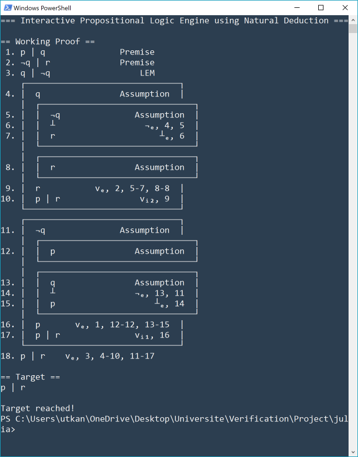
\includegraphics{example.png}
	\caption{Proof for the sequent $p \lor q, \neg q \lor r \seq p \lor r$.
	Note how closely it resembles the Proof~\ref{fig:proof}.}
	\label{fig:example}
\end{figure}

Following lines are the exact input we have provided to our program,
line-by-line, which brought us to the conclusion depicted in Figure~\ref{fig:example}:

\begin{center}
	\begin{tabular}{l}
		\verb^p | q, !q | r => p | r^\\
		\verb^LEM q^\\
		\verb^assume q^\\
		\verb^assume !q^\\
		\verb^nege 4 5^\\
		\verb^bote 6 r^\\
		\verb^conclude^\\
		\verb^assume r^\\
		\verb^conclude^\\
		\verb^ore 2 5-7 8-8^\\
		\verb^ori2 9 p^\\
		\verb^conclude^\\
		\verb^assume !q^\\
		\verb^assume p^\\
		\verb^conclude^\\
		\verb^assume q^\\
		\verb^nege 13 11^\\
		\verb^bote 14 p^\\
		\verb^conclude^\\
		\verb^ore 1 12-12 13-15^\\
		\verb^ori1 16 r^\\
		\verb^conclude^\\
		\verb^ore 3 4-10 11-17^
	\end{tabular}
\end{center}

\subsection{Implementation Details}

\section{Conclusion}

We are very content with the final version of our program. It is able
to produce proofs in a very appealing way, despite being a command-line
application. With the interactions of the user, it can prepare any
propositional logic proof using natural deduction, having a strict
enforcement on its validity at each and every step.

The software has an engine embedded within, and uses that engine at its
core to consume input and provide output through a monospace terminal.
Overall, the software is intended to be used as an interactive, stand-alone
command-line application. However, with only some minor modifications,
it can also be turned into a tool and a back-end engine for any other application.

\bibliography{ref} 
\bibliographystyle{plain}

\end{document}
